% Created 2020-03-14 Sat 13:57
% Intended LaTeX compiler: pdflatex
\documentclass[a4paper, 10pt]{article}
\usepackage[utf8]{inputenc}
\usepackage[T1]{fontenc}
\usepackage{graphicx}
\usepackage{grffile}
\usepackage{longtable}
\usepackage{wrapfig}
\usepackage{rotating}
\usepackage[normalem]{ulem}
\usepackage{amsmath}
\usepackage{textcomp}
\usepackage{amssymb}
\usepackage{capt-of}
\usepackage{hyperref}
\usepackage{minted}
\author{Anselm Coogan, Sean Wang}
\usepackage[utf8]{inputenc}
\usepackage[margin=3cm]{geometry}
\usepackage{fancyhdr}
\usepackage{caption}
\usepackage{bbold}
\usepackage{amsmath}
\usepackage{savesym}
\pagestyle{fancy}
\renewcommand{\listingscaption}{Algorithm}% Listing -> Algorithm
\date{\today}
\title{Implementing ORB-SLAM\\\medskip
\large Practical Course: Vision-based Navigation WS2019/20}
\hypersetup{
 pdfauthor={Anselm Coogan},
 pdftitle={Implementing ORB-SLAM},
 pdfkeywords={},
 pdfsubject={},
 pdfcreator={Emacs 26.3 (Org mode 9.1.9)}, 
 pdflang={English}}
\begin{document}

\maketitle

\section{Introduction}
\label{sec:org098c128}
Simultaneous Localization and Mapping (SLAM) is used by robots to map their environment in real-time and localize themselves in it simultaneously.
Originally, SLAM was developed using LiDARs \cite{slam}, however, the advent of small, mobile robots (i.e. drones) has required computational systems that rely on less expensive and heavy sensory equipment. 
This need was met with Visual SLAM - a SLAM system based on a monocular or stereo RGB camera setup.
One of the groundbreaking Visual SLAM systems is ORB-SLAM (OS) which was originally proposed in 2015 \cite{os} and further developed in \cite{os-II}.
The main contributions of OS are feature-reusing throughout the entire pipeline, local optimization, real-time capable tracking, mapping, loop closing, robust initialization and localization, and techniques for compact map representation to allow for long-term operation. 
The illumination, scale, rotation and translation invariant ORB features\cite{orb} are used for tracking, mapping, relocalization and loop closing - the main SLAM steps. 
Local pose tracking and map optimization are done through a novel, so-called Covisibility Graph. A subset of this graph, the Essential Graph, is exploited for real-time capable loop-closing. 
For monocular systems - with which the original OS paper concerned itself - the authors propose a heuristic algorithm for scene initialization that produces a unique, robust result. 
Furthermore, for scene recognition they propose a Bag of Words (BoW) \cite{bow} approach.
In our project we extended the stereo Visual Odometry (VO) system developed throughout the semester to an OS-like setup. 
Concretely, we implemented the Covisibility Graph used in tracking and mapping and the Essential Graph used in loop closing. 
Additionally, instead of the BoW approach of OS, we designed a place recognition system based on pose similarity and 3D-point correspondences. 
Finally, we adhered to the original authors’ suggestions for removing redundant keyframes whilst adding new keyframes more frequently than in the VO system. 
This added functionality results in increased computational time, though notwithstanding we were able to keep the system running in real-time at 20 Hz. 
Overall, our system was compared with its parent - the VO implementation - on the EUROC V1 1 dataset \cite{euroc} and showed improved map consistency and comparable pose and hence trajectory estimates. 
The implementation can be found on Gitlab.\footnote{https://gitlab.vision.in.tum.de/visnav\_ws19/w0031/visnav.git, branch: develop}

\section{System Overview}
\label{sec:orgb35b778}
As noted, the presented system was built based on and inspired by \cite{os} and \cite{os-II},
the main differences being that the original papers consider loop closures as disjunct from map building (operating in a separate thread), and that they use a more complex method for detecting loop closures - namely BoW versus pose similarity. 
The map representation is made up of 3D points in space, termed landmarks, keyframes (camera poses and associated landmark observations), and a Covisibility Graph connecting camera poses with each other based on 
similarity of viewpoints, see Figure \ref{fig:org80ff381}.
A high-level overview of the system flow is depicted in Figure \ref{fig:orgd992e0a}. It is divided into two main components: I) tracking and II) mapping with possible loop closure.
The tracking task consists of extracting features from the image frames, projecting a local map onto the current camera, matching existing landmarks in the map with detected features, 
and finally estimating the camera pose based on these matches.
This is done on a per-frame basis. If a frame is to be added as a new keyframe because it contains enough new information, the mapping part of the system is activated.
It is made up of several parts: first, it adds new observations of existing landmarks and creates new landmarks based on feature matches between the current left and right frames.
Then it necessarily adds the current frame as a keyframe and updates the covisibility graph. This is followed by detecting whether a loop closure can be performed.
Subsequently the local map is optimized using Bundle Adjustment (BA) \cite{ba} and finally, redundant keyframes are removed. The following sections discuss the methods (those that are different from VO) in more detail.

\begin{figure}[htbp]
\centering
\includegraphics[width=0.5\linewidth]{./resources/map-overview.png}
\caption{\label{fig:org80ff381}
The map is represented by landmarks (or map points), keyframes, and the Covisibility and Essential Graphs}
\end{figure}

\begin{figure}[htbp]
\centering
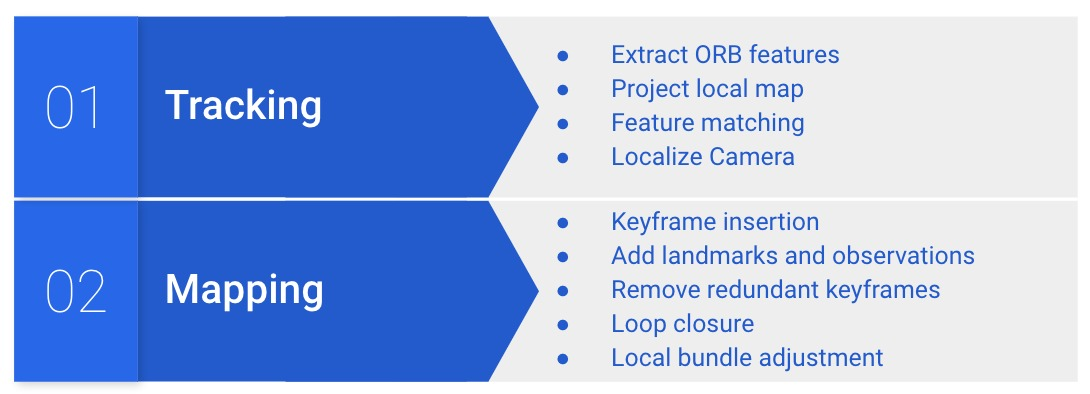
\includegraphics[width=0.7\linewidth]{./resources/system.jpeg}
\caption{\label{fig:orgd992e0a}
The system consists of two main parts, tracking and mapping. Tracking is done for every frame whereas mapping is done only if a frame is added as a keyframe}
\end{figure}

\section{Tracking}
\label{sec:orgd3e425f}
Odometry tracking is done for every frame. The pose estimate is initialized through the previous frame’s pose. Further pose estimation is conducted using ORB-features found in the left frame.
Features detected in the right frame are only used in mapping. However, since feature detection is computationally intensive, ORB-features are computed for both left and right frame concurrently, 
so that if mapping is concluded, the detected features are available without further computation by the mapping part. 2000 features are computed per frame. 

\subsection{Covisibility Graph}
\label{sec:orge25ac13}

The Covisibility Graph is one of the central contributions by the original Orb-SLAM authors. In contrast to visual odometry where tracking (and mapping) is done based on temporal proximity, the Covisibility Graph 
considers spatial closeness.
So instead of doing tracking and mapping by exploiting information only from the n previous keyframes and their associated landmarks, keyframes with similar scenes and poses are selected.
This is achieved by constructing a weighted, undirected graph where keyframes are nodes and an edge \(e_{ij}\) between two keyframes \(k_i\) and \(k_j\) exists if they have a similar view, 
i.e. share a minimum amount of landmark observations \(\theta_{min}=30\).
If an edge \(e_{ij}\) exists, its weight is equal to the number of shared landmarks. See Equations \ref{eq:cov-edge-1} and \ref{eq:cov-edge-2} where \(obs_i\) are the unique landmark IDs observed by keyframe \(i\).
\begin{equation}
\label{eq:cov-edge-1}
\widehat{e}_{ij} = \sum_{obs_i}\sum_{obs_j}\mathbb{1}_{obs_i=obs_j}
\end{equation}

\begin{equation}
\label{eq:cov-edge-2}
e_{ij} = 
\begin{cases}
\widehat{e}_{ij}, & \text{if } \widehat{e}_{ij} \geq \theta_{min} \\
0 & \text{else}
\end{cases}
\end{equation}

A visualization of the graph can be seen in Figure \ref{fig:org7838166}. The Covisibility Graph is used to construct a local map in which the current frame can be localized.
A subset of this graph, the Essential Graph, is used later on in the system when propagating pose updates during loop closure. An edge in the Essential Graph exists if the number of shared landmarks is 
equal to or greater than \(\theta_{min}^{EG} \geq \theta_{min}\), in our case \(\theta_{min}^{EG}=60\). A graphical representation is given in Figure \ref{fig:org293b31c}.

\begin{figure}[htbp]
\centering
\includegraphics[width=0.5\linewidth]{./resources/cov-graph.png}
\caption{\label{fig:org7838166}
The Covisibility Graph. Nodes are keyframes and edges between keyframes with number of shared observations exceeding \(\theta_{\text{min}}\).}
\end{figure}

\begin{figure}[htbp]
\centering
\includegraphics[width=0.5\linewidth]{./resources/essential-graph.png}
\caption{\label{fig:org293b31c}
The Essential Graph. A subset of the Covisibility Graph. For an edge to exist, keyframes must share more than \(\theta_{\text{min}}^{\text{EG}}\) landmark observations.}
\end{figure}

\subsection{Local Map}
\label{sec:org77aa4ac}
To generate a local map, two steps are necessary. First, the landmarks seen by the most recent keyframe are projected into the current frame and matched with the current frame’s ORB-features.
Based on this matching, the current pose is calculated in an initial estimation. Second, the matches are used to find the keyframe(s) k\(_{\text{1}}\) that share at least \(k_1^{min}=10\) landmark observations with the current frame.
Then, the local map is created by combining all landmarks seen by the keyframes in k\(_{\text{1}}\) and by the set of neighbors of k\(_{\text{1}}\) in the Covisibility Graph.
This local map is then projected into the current frame, and the current pose is estimated based on matched ORB-features. A graphical abstraction of the local map is given in Figure \ref{fig:orgbf8dbd9}.

\begin{figure}[htbp]
\centering
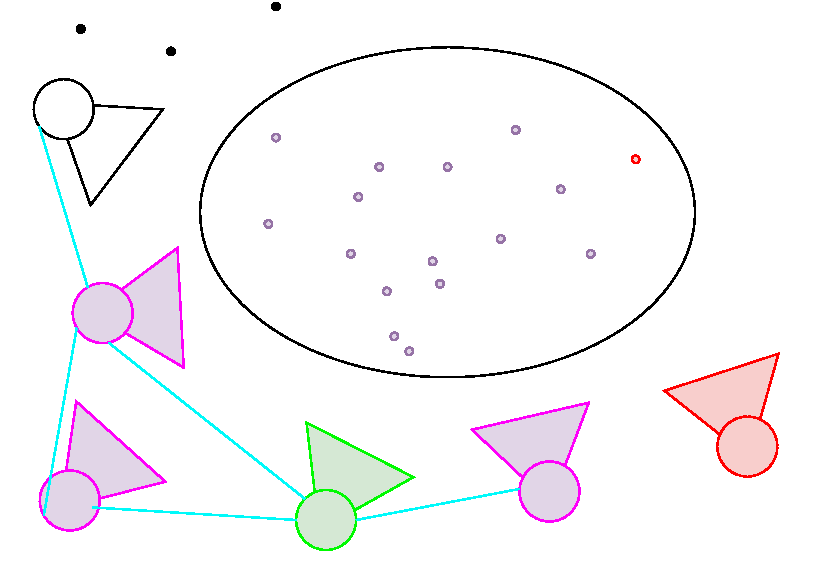
\includegraphics[width=0.5\linewidth]{./resources/local-map.pdf}
\caption{\label{fig:orgbf8dbd9}
The local map used to localize the current frame. The current frame is highlighted in red, the (single) k\(_{\text{1}}\) frame is in green, k\(_{\text{1}}\)'s neighbors in the Covisibility Graph are in purple, and a not-included keyframe is given in white. The shared point between k\(_{\text{1}}\) and the current frame is red and the local map consists of the red point and the points seen by the neighbors, highlighted in purple.}
\end{figure}

\subsection{Keyframe Decision}
\label{sec:org7ede62f}
Tracking is completed by deciding whether to add the current frame as a keyframe. Overall, the high-level goal is to add only keyframes with enough new information.
If the mapping thread is currently busy, the frame is discarded regardless of its potential value. If it is not, the frame is selected as a keyframe if either of the following conditions hold:
\begin{itemize}
\item there were more than \(m_{min}=130\) matches with the local map and more than \(f_{min}=50\%\) features of the frame are unmatched
\item the current number of keyframes is less than or equal to \(kf_{min}=5\) ,
\item more than \(kf_{max}=40\) frames have passed since the last keyframe insertion
\end{itemize}
The first part of the first condition ensures good tracking, whereas the second part asserts that only keyframes with new information are being added.
However, this can result to losing track if too rapid changes occur. To combat this, the second condition is introduced: if too much time has passed since the last insertion (and hence tracking was lost because condition one didn't
hold) the keyframe is inserted regardless. Finally, the third conditions ensures that aggressive keyframe removal, especially in the beginning, doesn't become a problem.

\section{Mapping}
\label{sec:org8eb8273}
If a frame was selected to be added as a keyframe, the mapping part of the system comes into play. First, feature descriptors between the left and right frame are matched. 
As previously mentioned, ORB-feature detection for the right image is done concurrently to tracking so that both feature sets are available at this point. 
New landmarks are added based on stereo matches that have not yet been associated with an existing landmark in the preceding tracking step and observations of existing landmarks are added as well. 
In order to disregard outliers as quickly as possible, the distance to the left camera needs to be between \(d_{min}=0.1m\) and \(d_{max}=10m\).
Once this is completed, further mapping steps, namely redundant keyframe removal, loop closure and local bundle adjustment, are computed in a separate thread.

\subsection{Keyframe Removal}
\label{sec:orgf86bb38}
Keyframes with redundant information produce two undesirable effects. First, they unnecessarily inflate the system’s memory footprint. Second, the redundant keyframes' pose estimates are 
likely to have an adverse outcome on pose and map estimation.
Thus, keyframes are removed if more than \(k_{max}^{overlap}=90\%\) of the landmarks they observe, are also seen by at least three other keyframes. For better understanding, pseudo-code for this procedure 
is given in Algorithm \ref{orga351904}.

\begin{listing}
\begin{minted}[escapeinside=||,mathescape=true]{text}
FOR keyframe in keyframes
    SET overlapCounter to 0
    FOR landmark in landmarks of keyframe:
        IF observationCount of landmark > 3 THEN
           INCREMENT overlapCounter
        END IF
    END FOR
    SET overlapPercentage to (DIVIDE overlapCounter by (SIZE of landmarks))
    IF overlapPercentage > 0.9 THEN
       REMOVE keyframe from keyframes
    END IF
END FOR
\end{minted}
\caption{\label{orga351904}
The algorithm used for keyframe removal.}
\end{listing}

\subsection{Loop Closure}
\label{sec:orgb749bc5}
Every estimation step will introduce an error - however slight it may be. As time progresses, the error will accumulate and cause a problem known as drift, as exemplified in Figure \ref{fig:org756346f}.
This error is present in both the map and the pose estimates. A technique known as loop closure is used to combat this.
\begin{figure}[htbp]
\centering
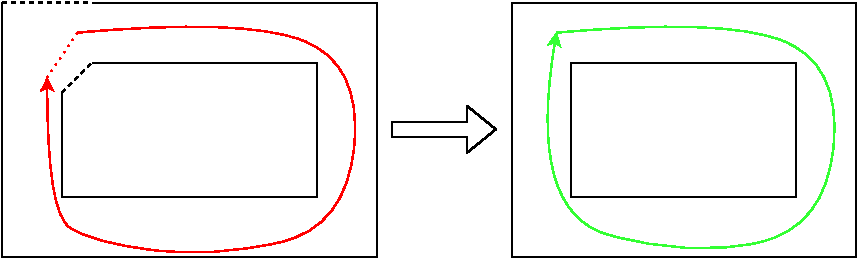
\includegraphics[width=0.5\linewidth]{./resources/drift.pdf}
\caption{\label{fig:org756346f}
Accumulated error in map and trajectory estimation known as drift seen on the left. To combat this, previously seen places (e.g. landmarks) need to be recognized so that they aren't added as new landmarks. Once this happens, drift can be corrected via loop closure (right).}
\end{figure}
The main idea is to recognize a previously explored place and then correct the error that has accumulated in between viewings. 
In OS this is achieved by recognizing places based on the BoW feature representations between frames. Our system uses a simpler, but possibly more intuitive, method based on pose similarity.
In the first step, possible loop closure candidates are identified. This is done by first computing the absolute pose difference \(p\) between the current keyframe and all its neighbors 
in the covisibility graph as given by Equation \ref{eq:pose-diff}, where \(A\) and \(B\) are the poses, \(I\) is the identity matrix and \(\|*\|_{\rm {F}}\) is the Frobenius norm. 
\begin{equation}
\label{eq:pose-diff}
p = \|(A^{-1} B) - I\|_{\rm {F}}
\end{equation}
The largest pose difference is then compared to the pose differences between the current keyframe and all other non-neighboring keyframes; 
keyframes with smaller pose differences are considered as loop closure candidates. For each candidate, its ORB descriptors are matched with those of the current keyframe - only features that are associated with an 
existing landmark are considered. This results in 3D-3D correspondences and the resulting point clouds are aligned using RANSAC \cite{ransac}.
If this alignment is supported by enough inliers \(n_{min}^{inliers}=12\) and it has more inliers than its competing loop closure candidates, it is accepted as a loop closure keyframe.
Closing a loop is composed of two steps. First, landmarks are merged: from the matched 3D points between the loop closure frame and the current keyframe the both observations are 
counted towards the associated landmark of the loop closure frame. This landmark gets new observations from the current keyframe and its neighbors in the Covisbility Graph that previously observed the erroneous landmark. 
The second part is correcting the drift. This is done by updating the pose of the current keyframe based on the new landmark matches and then propagating this result using Breadth-First Search (BFS) \cite{bfs} through the Essential Graph. 
The algorithm is given in Algorithm \ref{orga29b42d}. This feature is accomplished by keeping the relative poses between landmarks constant and only updating their poses w.r.t. the world coordinate system.
However, the pose update is done separately from loop closure detection after the map has been optimized with local BA and in the main thread (not the separate mapping thread).

\begin{listing}
\begin{minted}[escapeinside=||,mathescape=true]{text}
CREATE queue
ADD currentFrame to queue
ADD neighbors of currentFrame to queue

CREATE visited
ADD currentFrame to visited
ADD neighbors of currentFrame to visited

WHILE queue not empty DO
      SET currentNode to queue.popFront()
      FOR neighbor of neighbors in essentialGraph of currentNode
          IF neighbor in visited
             CONTINUE WHILE
          END IF
          SET relativePose to RELATIVE_POSE between neighbor and currentNode
          SET absolutePose of neighbor to currentNode.pose TIMES (INVERSE of relativePose)
          ADD neighbor to visited
          ADD neighbor to queue
      END FOR
END WHILE

\end{minted}
\caption{\label{orga29b42d}
Breadth-First Search applied to pose update propagation via the Essential Graph.}
\end{listing}

\subsection{Local Bundle Adjustment}
\label{sec:org18fc06c}
After redundant keyframes have been removed and a possible loop closure has been found, the map and keyframe poses are optimized using Bundle Adjustment (BA). Again, the Covisibility Graph is used to ensure spatially local map optimization. 
The optimization is thus done on the current keyframe and its neighbors in the Covisibility Graph plus all landmarks observed by these keyframes.
Non-neighboring Keyframes that observe any of the optimized landmarks are also included but kept fixed during optimization.

\section{Evaluation}
\label{sec:orgbfee33d}
In the scope of this project, the developed system was evaluated on the first route of the EUROC V1 dataset \cite{euroc} and compared against the precedingly developed Visual Odometry system.
This was done on an eight-core 2.3 GHz Intel Core i9 processor running with 32 GB RAM.

\subsection{Real-time Capability}
\label{sec:org5dffd49}
The system should be able to run in real-time. For the considered dataset, this evaluates to a framerate of 20Hz or 50ms of computation time per frame. 
On average, our system is able to achieve this, running at 30.48 per frame. However, around 1\% of frames exceed the real-time threshold, with single spikes at up to 61.0 ms.
The most computationally intensive tasks are ORB feature extraction and local map localization with maximum runtime values of 26.1ms and 30.0ms, respectively.
Hence, significant speed-up is achieved by running ORB-feature extraction in multiple threads.
Optimizing the ORB-feature extraction algorithm and the data structures and routines used throughout the system should be able to bring down the worst-case 
runtimes so that the real-time constraint is achieved for all frames.
A detailed timing analysis can be found in Table \ref{tab:orgc29221d}. 

\begin{table}[htbp]
\caption{\label{tab:orgc29221d}
Timing analysis for the different functionalities of our system (\(\sigma\) is the standard deviation, \(\sigma^{\text{2}}\) the variance). A distinction is made between the main thread that processes ever frame, a separate thread for ORB-feature extraction in the right frame that is also run every frame, and finally the separate mapping thread. Note that only the main subtasks are considered.}
\centering
\begin{tabular}{lrrrrr}
Step & Avg. t [ms] & min. t [ms] & max. t [ms] & \(\sigma\)  [ms] & \(\sigma^{\text{2}}\) [ms\(^{\text{2}}\)]\\
\hline
\hline
\textbf{MAIN THREAD} & \textbf{3.05E1} & \textbf{1.93E-2} & \textbf{6.10E1} & \textbf{7.99} & \textbf{6.39E1}\\
BFS pose update & 1.83E-2 & 4.76E-2 & 4.70E-4 & 1.07E-2 & 1.13E-4\\
\hline
\emph{Tracking} & \emph{2.90E1} & \emph{1.14E1} & \emph{5.70E1} & \emph{7.42} & \emph{5.50E1}\\
ORB (left) & 1.35E1 & 6.82 & 2.6E10 & 2.85 & 8.14\\
Tracking (prev. landmarks) & 4.72 & 1.44E1 & 1.90E-2 & 1.77 & 3.13\\
Tracking (local map) & 1.07E1 & 3.57E-3 & 3.00E1 & 4.49 & 2.02E1\\
Keyframe decision & 2.33E-4 & 1.04E-3 & 1.18E-4 & 9.60E-5 & 9.21E-9\\
\hline
ORB (right) (separate thread) & 1.34E1 & 2.66E1 & 6.70 & 2.90 & 8.35\\
\hline
\emph{Mapping} & \emph{8.19} & \emph{9.39E-1} & \emph{2.01E1} & \emph{4.27} & \emph{1.82E1}\\
Stereo ORB matching & 1.57 & 1.39E-1 & 1.30E1 & 1.77 & 3.12\\
Adding landmarks \& observations & 4.21E-1 & 7.03E-2 & 1.22 & 2.82E-1 & 8.00E-2\\
Adding keyframe & 1.36 & 4.88E-2 & 3.04 & 7.44E-1 & 5.54E-1\\
\hline
\hline
\textbf{MAPPING THREAD} & \textbf{8.74E1} & \textbf{2.14E-1} & \textbf{2.67E2} & \textbf{4.88E1} & \textbf{2.38E2}\\
Detecting loop closure & 6.27 & 3.90E-3 & 1.57E2 & 2.20E1 & 4.87E2\\
Local bundle adjustment & 6.77E1 & 1.46E-1 & 1.85E2 & 3.74E1 & 1.40E3\\
Removing redundant keyframes & 8.63 & 5.16E-4 & 2.04E1 & 5.14 & 2.64E1\\
\end{tabular}
\end{table}

\subsection{Map Consistency}
\label{sec:org29d5359}

Map consistency is somewhat more difficult to evaluate quantitatively as no ground truth map of the environment exists. 
Hence, other heuristics are considered. Since the scene under consideration is indoors and does not exhibit long hallways, one such heuristic are the distances of the map points 
to the origin (the first frame pose) and the underlying distribution. Both systems create a similar amount of points (OS: 21563, VO: 20630). 
Additionally, the most extreme outliers have similar distances of \(2.07 \cdot 10^7\) and \(2.49 \cdot 10^7\) for OS and VO, respectively. Furthermore, due to these similarities the distributions are very similar on the
surface as well with standard deviations being \(2.28 \cdot 10^5\) and \(2.50 \cdot 10^5\), variances of \(5.21 \cdot 10^{10}\) and \(6.26 \cdot 10^{10}\), and medians lying at 4.32 and 4.24, for OS and VO, respectively.
However, as indicated by the slightly higher variance and standard deviation of the VO system, our system exhibits fewer outliers. Again, defining outliers is a bit tricky with no ground truth available. However,
qualitatively inspecting the (non-symmetric) map makes it possible to consider points with distances greater than \(6.9m\) to be outliers and points with distances greater than \(50m\) to be extreme outliers. For these metrics
our system shows significant improvement with 7 vs. 17 extreme outliers and 95 vs. 125 regular outliers (note that these contain the extreme outliers).
A layover of both maps with highlighted outliers depicts this difference in Figures \ref{fig:orgbe7c521} and \ref{fig:org5ed7aad}.
\begin{figure}[htbp]
\centering
\includegraphics[width=0.75\linewidth]{./resources/maps-topview.png}
\caption{\label{fig:orgbe7c521}
The resulting maps from the EUROC V1 1 dataset for our system (red) and VO (lightgreen) seen in a birds-eye view. Outliers are marked in bold in the respective colors.}
\end{figure}

\begin{figure}[htbp]
\centering
\includegraphics[width=0.75\linewidth]{./resources/maps-sideview.png}
\caption{\label{fig:org5ed7aad}
The resulting maps from the EUROC V1 1 dataset for our system (red) and VO (lightgreen) as viewed from the side. Outliers are marked in bold in the respective colors.}
\end{figure}


\subsection{Trajectory Accuracy}
\label{sec:orgd272649}
For the trajectory a ground truth exists, and hence, evaluation is more straightforward. 
Two common metrics to evaluate trajectory estimates are the Absolute Trajectory Error (ATE) and Relative Pose Error (RPE) \cite{pose-errors}.
ATE is a metric to calculate global consistency of the estimated trajectory.
It is computed by first aligning the estimated trajectory \(E\) with the ground truth trajectory \(G\) through least-squares minimization. The resulting rigid body translation \(T\) is then used to compute the remaining
error between the trajectories. The formal definition is given in \ref{eq:ape}\cite{pose-errors} with \(n\) being the number of frames in the trajectories and \(G_i\) and \(E_i\) the poses
for frame \(i\) for the ground truth and estimated poses, respectively. The \(trans()\) operator returns the translational component of a transformation.
\begin{equation}
\label{eq:ape}
ATE = (\sum_{i=1}^{n} \|\text{trans}(G_i^{-1}TE_i)\|^2)^{\frac{1}{2}}
\end{equation}
Note that ATE does not take rotational errors into consideration.
The Relative Pose Error is a measure for drift. A single error is computed over an interval \(\Delta\) and given in Equation \ref{eq:rpe-1}. For a single pose \(i\) the error is then computed
for a given interval \(\Delta\) and all pose error are averaged as given by \ref{eq:rpe-2} with \(m=n-\Delta\). Again, only the translational component is considered.

\begin{equation}
\label{eq:rpe-1}
RPE_i = (G_i^{-1}G_{i+\Delta})^{-1}(E_i^{-1}E_{i+\Delta})
\end{equation}

\begin{equation}
\label{eq:rpe-2}
RPE_{\Delta} = (\frac{1}{m} \sum_{i=1}^m\|\text{trans}(RPE_i)\|^2)^{\frac{1}{2}}
\end{equation}

\begin{equation}
\label{eq:rpe-3}
RPE = \frac{1}{n}\sum_{\Delta=1}^{n}RPE_\Delta
\end{equation}

Finally all possible time intervals \(\Delta\) are taken into account and an overall average is computed, see Equation \ref{eq:rpe-3}.
Instead of using the trajectory of the non-optimized first pose estimates for every frame, only the final keyframe poses are used for the path.
Necessarily, this results in less smooth trajectories. Although local BA, loop closure and local map localization are in use, based on the Absolute Trajectory and Relative Pose Error, no significant improvement of 
our system compared to VO can be seen.
APE for our system and VO is 0.089761 and 0.106138 respectively, a mere 15\% decrease. For RPE, the values come out to 0.256769 and 0.253313 for our system and VO, respectively.
Here the error even increased by 1.3\%.
This is likely due to the map being a closed room where even a VO system accumulates no significant drift (as it would in looping hallways). The poses are depicted in Figures \ref{fig:org017330f} and \ref{fig:orgfea4b18}

\begin{figure}[htbp]
\centering
\includegraphics[width=0.5\linewidth]{./resources/traj-os.png}
\caption{\label{fig:orgfea4b18}
The trajectory of our system on the EUROC V1 1 dataset compared to the ground truth trajectory.}
\end{figure}

\begin{figure}[htbp]
\centering
\includegraphics[width=0.5\linewidth]{./resources/traj-vo.png}
\caption{\label{fig:org017330f}
The trajectory of the VO system compared to the ground truth trajectory is qualitatively as well as quantitatevly very similar to our system's result.}
\end{figure}

\section{Conclusion}
\label{sec:org8df3246}
During the final stretch of the semester we were able to extend the hitherto developed Visual Odometry system to include a large part of the contributions of ORB-SLAM: the Covisibility Graph for local tracking
and mapping, Loop Closure for drift compensation via the Essential Graph and BFS pose update propagation, and finally Keyframe Removal for compact map representation. Through performance optimization (most notably
by running feature detection for left and right frames concurrently) we were able to withstand the added functionality and keep the system running at 20 Hz for 99\% of the time. 
Evaluating the previous VO system to ours showed improved map consistency and similar numerical results for trajectory accuracy, 
likely due to the map at hand. Comparing the systems on different datasets from the EUROC datasets was not possible as both systems weren't robust enough
to manage the more difficult tracks (although notably VO failed far sooner than our OS system). There are two performance improvements that the timeframe did not permit to implement but would likely result in a comparable
system to the original ORB-SLAM: first, using a BoW representation of the ORB-feature space for place recognition in Loop Closure, and secondly, to run Loop Closure truly in a third thread (instead of having it be part
of mapping).


\bibliographystyle{plain}
\bibliography{bib}
\end{document}
